\section{Case Analysis}
We further demonstrate how set-RNN works with two examples.
In the first example from the RCV1-v2 dataset, the most probable set predicted by set-RNN (which is also the correct set in this example)  does not come from the most probable sequence. Top sequences in decreasing probability order are listed in Table~\ref{tab:pred_case_study}. The correct label set \{forex, markets, equity, money markets, metals trading, commodity\} has the maximum total probability of 0.161, but does not match the top sequence.

% \small{
% \texttt{  \footnotesize{  \linespread{0.1}
% FOCUS-Dollar romps, weak Dow blunts share rallies. The dollar romped ahead against the mark on Tuesday and European bourses also prospered, with British blue chips breaking records, but share rallies were blunted by a weaker Wall Street start.The dollar sneaked above the psychological 1.50 marks barrier in early European trade. It continued to firm as the day progressed and a wave of fund buying propelled its towards 1.51."Once we moved beyond 1.50, it\'s momentum-driven," said Keld Holm, international economist at Lehman BrothersIt is now trading above levels seen on July 16, when dollar/mark suffered its biggest one-day drop this year as New York share prices crashed.The dollar also rallied to 1.2345 Swiss francs --  up sharply from its 1.2157 close in Europe on MondayThe dollar rally began on Monday after Bundesbank council member Ernst Welteke said there was room for further German interest rate cuts if M3 money supply growth continued to slow....
% His comment knocked the mark across the board and the dollar was further spurred overnight by Wall Street\'s strong Monday performance and a jump in Treasuries.On the bourses, leading shares in London, Frankfurt and Paris all got an early leg-up by the overnight surge on the Dow, which posted its biggest one-day gain in over a month to close 1.3 percent up.Im morning trading Tuesday London\'s blue-chip FTSE 100 index jumped more than 20 points to a record 3,933.6, surpassing its previous record of 3,922.1 set on August 28. However, after a weaker start on Wall Street Tuesday, it fell back sharply to close just below its record closing high at 3,916.1, up just 5.3 points. Analysts said London\'s gains had also been held in check by a lacklustre performance by government bonds, overshadowed by worries that Britain will cut interest rates further to stoke pre-election growth regardless of the inflation risk.In Frankfurt, German shares ended a lively floor trade session higher, with the 30-share DAX index closing at 2,570.95 points, up 22.22. In later electronic trading German shares fell back slightly under the influence of New York but dealers said the ever strengthening dollar (which would make German goods cheaper for foreigners) and firm government bonds were continuing to provide support.The same motors, plus gains in the French franc, propelled Paris shares, which started firmer and quickly strengthened. However, the main CAC-40 index fell back after Wall Street\'s York\'s shaky start to finish just off the day\'s high, up 21.82 points or 1.08 percent at 2,042.12.Stock and currency markets remained gripped by interest rate prospects following last Friday\'s U.S. jobs data showing lower unemployment and stronger earnings.U.S. producer and consumer price data -- due Thursday and Friday -- will be scrutinized for fresh signs of inflation pressures. Many traders and investors are betting on a rise of 0.25 percentage point in U.S. interest rates when the Federal Open Market Committee next meets on September 24.Opinions are mixed as to whether the central bank will decide this time to raise or leave interest rates unchanged, perhaps until after the November 5 presidential election.CURRENCIES AT 1600 GMTThe dollar was at 1.5088 marks and 109.85 yen compared with late European levels on Monday of 1.4935 and 109.15.STOCK MARKETSThe Financial Times-Stock Exchange index of 100 leading British shares closed up 5.3 points at 3,916.1.In Paris, the CAC-40 share index closed up 21.82 at 2,042.12.The 30-share DAX index in Frankfurt closed up 22.22 at 2,570.95.PRECIOUS METALSGold closed unchanged from Monday\'s close at 383.45. Silver finished at \$5.11, up two cents.'
% }
% }



% bag of words set:
% \texttt{  \footnotesize{  \linespread{0.1}
% foreign, monday, blu, begin, govern, data, shaky, surpass, live, sneak, pari, econom, clos, support, point, pre, im, french, trad, rate, barry, treasur, leav, low, dollar, council, unemploy, metal, britain, produc, show, meet, job, street, weltek, inflat, strong, swiss, propel, knock, percent, earn, firm, germ, romp, wall, progress, decid, dax, anal, frankfurt, suff, cent, franc, year, cut, brother, prec, sign, continu, grip, novemb, overnight, bundesbank, spur, open, move, index, level, growth, silf, fts, lacklustr, gmt, strength, record, bet, lead, floor, time, mark, keld, electron, prospect, stock, prosp, gain, presid, cac, motor, ernst, remain, commit, held, thursday, perform, sharp, july, compar, memb, fresh, elect, good, pric, overshadow, break, buy, morn, early, bours, septemb, stok, back, opinion, rise, pressur, post, lehm, deal, european, start, due, risk, exchang, comment, scrutin, focus, session, month, worry, big, late, chip, tuesday, cheap, unchang, m3, slight, psych, feder, interest, dow, europ, set, suppl, drop, jump, fund, market, rais, wav, room, weak, financ, momentum, board, brit, mix, leg, driv, high, consum, main, prev, finish, intern, york, make, check, slow, bond, holm, currenc, quick, day, crash, london, ahead, yen, money, bank, end, fell, august, invest, friday, influ, gold, provid, surg, shar, rally, blunt
% }
% }


\begin{table}[h]
\resizebox{1.01\columnwidth}{!}{%resize the table
\begin{tabular}{l|l}
PROB	& SEQUENCE\\
\hline
0.0236 	& equity, markets, money markets, forex\\
0.0196	& {\bf forex, markets, equity, money markets, metals trading, commodity}\\
0.0194	& {\bf equity, markets, forex, money markets, metals trading, commodity}\\
0.0159	& {\bf markets, equity, forex, money markets, metals trading, commodity}\\
0.0157	& {\bf forex, money markets, equity, metals trading, markets, commodity}\\
0.0153	& {\bf forex, money markets, markets, equity, metals trading, commodity}\\
0.0148	& markets, equity, money markets, forex\\
0.0143	& {\bf money markets, equity, metals trading, commodity, forex, markets}\\
0.0123	& {\bf markets, money markets, equity, metals trading, commodity, forex}\\
0.0110 	& {\bf markets, equity, forex, money markets, commodity, metals trading}\\
0.0107	& {\bf forex, markets, equity, money markets, commodity, metals trading}\\
0.0094	& {\bf forex, money markets, equity, markets, metals trading, commodity}\\
\hline
\end{tabular}
}
\caption{The set-RNN predicted set (also the correct set) \{forex, markets, equity, money markets, metals trading, commodity\} has the max total probability of 0.161, but does not match the top sequence. Sequences for the correct set are in bold.}\label{tab:pred_case_study}
\end{table}

%%%%%%%%%%%%%%%%%%%%%%%%%%%%%%%%%%%%%%%%%%%%%%%%%%%%%%%%%%%%%%%%%%%%%%%%%%%%%%%%
%%%%%%%%%%%%%%%%%%%%%%%%%%%%%%%%%%%%%%%%%%%%%%%%%%%%%%%%%%%%%%%%%%%%%%%%%%%%%%%%
Next we demonstrate the issue with prescribing the sequence order in seq2seq-RNN with a TheGuardian example\footnote{\scriptsize This document can be viewed at \url{http://www.guardian.co.uk/artanddesign/jonathanjonesblog/2009/apr/08/altermodernism-nicolas-bourriaud}}. Figure~\ref{fig:models} shows the predictions made by seq2seq-RNN and our method. In this particular example the top sequence agrees with the top set in our method's prediction so we can just analyze the top sequence. seq2seq-RNN predicts \texttt{Tate Modern} (incorrect but more popular label) while we predict \texttt{Tate Britain} (correct but less popular label). The seq2seq predicted sequence is in the decreasing label frequency order while our predicted sequence is not. In the training data, \texttt{Exhibition} is more frequent than \texttt{Tate Britain} and \texttt{Tate Modern}. If we arrange labels by decreasing frequency, \texttt{Exhibition} is immediately followed by \texttt{Tate Modern} 19 times, and by \texttt{Tate Britain} only 3 times. So it is far more likely to have \texttt{Tate Modern} than \texttt{Tate Britain} after \texttt{Exhibition}. However,  at the set level, \texttt{Exhibition} and \texttt{Tate Modern} co-occurs 22 times while \texttt{Exhibition} and \texttt{Tate Britain} co-occurs 12 times, so the difference is not so dramatic. In this case, imposing the sequence order biases the probability estimation and leads to incorrect predictions.
%
% In the second case analysis present a case analysis document  to show how the set-model is superior to the sequence-model for multilabel text classification.  Ground Truth Label (sorted by frequency): ‘Culture’ ‘Art and Design’ ‘Art’ ‘Exhibitions’ ‘Tate Britain’. Extracted keywords by attention (over all steps): Tate, Curators, Newspapers, Exhibition, Philosophers, Art, Britain, Science, Doctor, Journalistic, Reviews, Artwork, Delta, Avant, Fashion, Literature, Grade, Manifesto.
%
%
% Top word evidences extracted by attention show that keywords are good enough for text multilabel prediction task (from this example, we show that ground truth labels can be inferred by these keywords). We don’t have to encode the documents as a sequence. We can use bag of words to represent the document.
% In Figure~\ref{fig:models} $h$ is the hidden history state. $h_0$ is the initial hidden state, which is randomly initialized by the model. $SOS$ is the start of the sentence symbol and $EOS$ is the end of the sentence symbol.
% In the training set, Frequency of bigram (exhibition, tate modern)=19, Frequency of bigram (exhibition, tate british)=3
%  ``Tate modern'' is associated with exhibition, and ``tate britain'' is associated with ``painting and art''
% So it is very likely to predict tate modern after exhibition, if we sort the labels by frequency. 
% Our set prediction method can learn the optimal order and then make predictions. It is easy to predict ``tate britain'' given label ``art'' as history and top evidences extracted by attention mechanism.

% Set prob of culture art and design art exhibition tate modern = 0.095
% Set prob of the other one = 0.07
%  \begin{figure}[h]
% 
\includegraphics[width=\columnwidth]{figs/docexample.png}
% \caption{\fontsize{10}{12}\selectfont  Example document (text shown incomplete). Ground Truth Label (sorted by frequency): ‘Culture’ ‘Art and Design’ ‘Art’ ‘Exhibitions’ ‘Tate Britain’.\\
% Extracted keywords by attention (over all steps): Tate, Curators, Newspapers, Exhibition, Philosophers, Art, Britain, Science, Doctor, Journalistic, Reviews, Artwork, Delta, Avant, Fashion, Literature, Grade, Manifesto.}
% \label{fig:example}
% \end{figure}
% \begin{figure}[t]
% \hspace{-2ex}
% 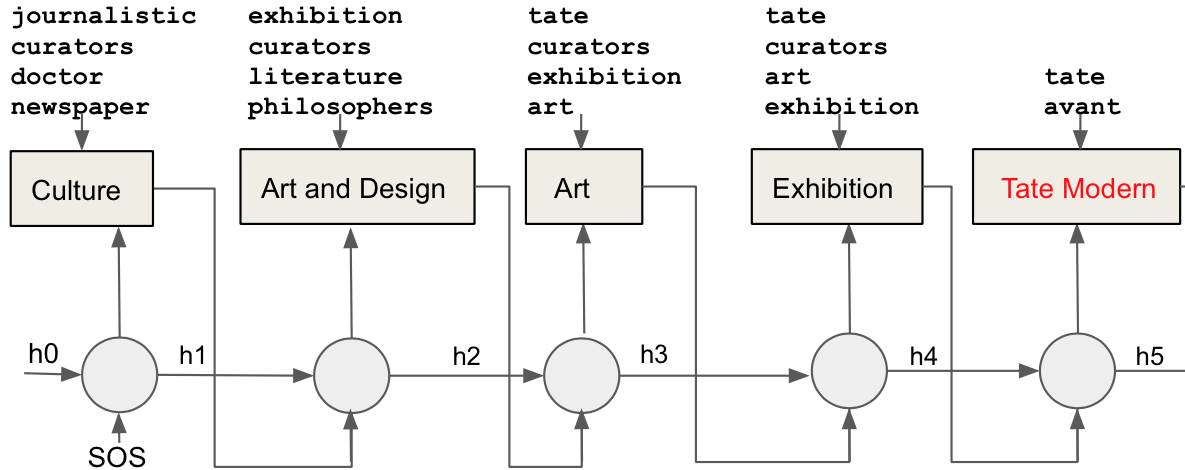
\includegraphics[width=1.2\columnwidth]{figs/train_sequence.png}
%
% \label{fig:models}
% \end{figure}
\begin{figure}[t]
%\hspace{-2ex}
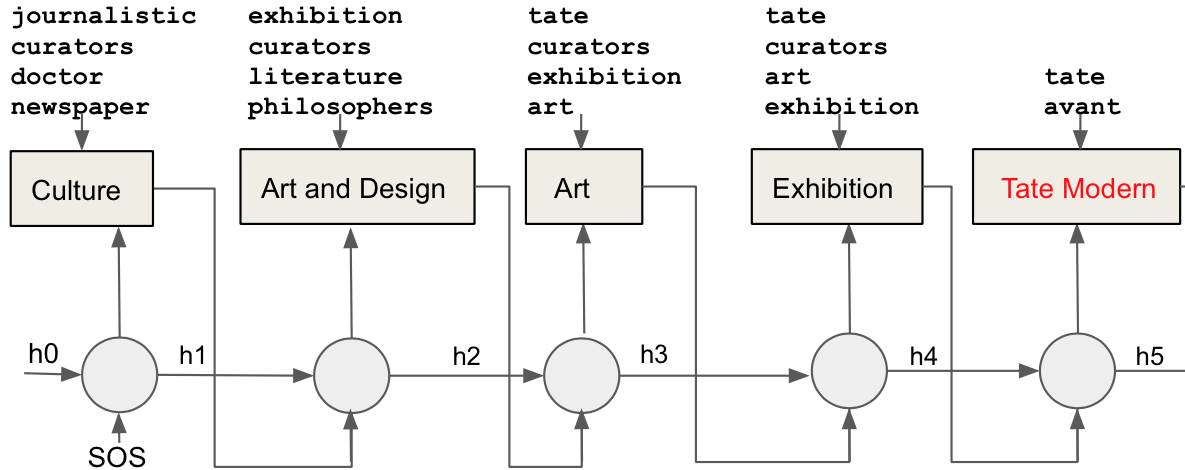
\includegraphics[width=1.0\columnwidth]{figs/train_sequence.png}
%\vspace{-4ex}
%\hspace{-2ex}
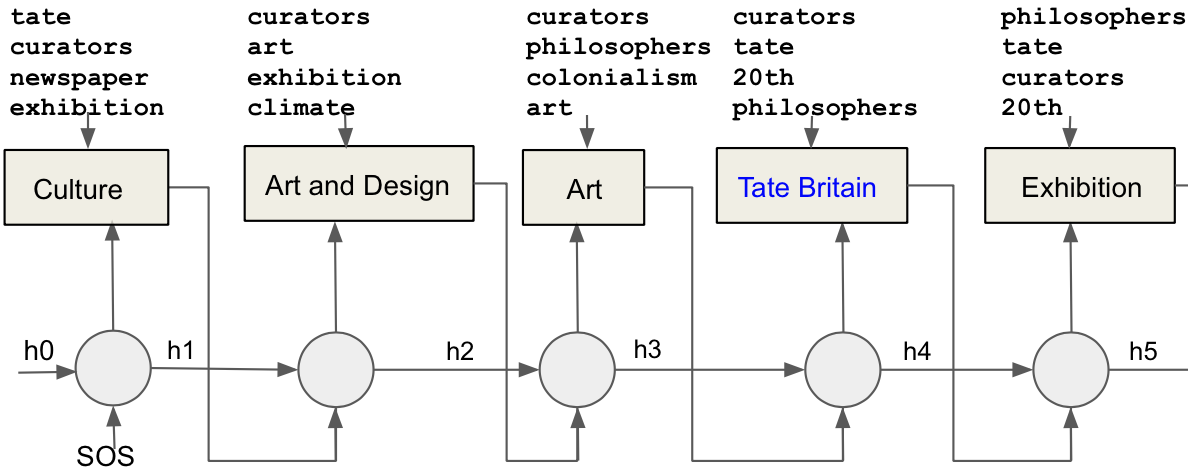
\includegraphics[width=1.0\columnwidth]{figs/train_set.png}

\caption{\fontsize{10}{12}\selectfont  Top: best sequence by seq2seq-RNN; bottom: best sequence by set-RNN. Above models, at each time, we list the top unigrams selected by attention.\vspace{2ex}}
\label{fig:models}
%\vspace{-6ex}
\end{figure}